\documentclass{article}
\usepackage{geometry}
\geometry{a4paper, top=3cm, bottom=3cm, left=2cm, right=2cm}
\usepackage[utf8]{inputenc}
\usepackage[english]{babel}
\usepackage{hyperref}
\usepackage{amssymb}
\usepackage{amsmath}
\usepackage{txfonts}
\usepackage{mathdots}
\usepackage{graphicx}
\usepackage[section]{placeins}
\usepackage{wrapfig}

\makeindex


\title{Advanced Database and Information Systems}
\author{Riccardo Salvalaggio}
\date{19th of April, 2021}


\begin{document}

\maketitle
\newpage
\tableofcontents
\newpage

\section{Semi-structured Data models: XML, XPath, XRel}

Structured Data models are obsolete nowadays: inadequate representation, semantic overloading, difficulty on recursion, rigid schema, limited throughput.
Now, semi-unstructured data format: data is no longer dependent on a schema (such as tables), is self-descriptive (good labels), more scalability. This needed is born because data is interlinked between each other (e.g. IoT, smart systems) and generated from DBs.
Anyway, a standardized representation is needed: a new language to structure in a flexible way data and semantically annotate it.

\subsection{XML}

Extensible Markup Language, derived from HTML structure (use of tags), born in late 90s use a tree-structure to describe and organize data.
Start- and end-tag with the inner part of the document are called \textit{element, }the name of it is the name of the tag and the content is the enclosed part. If an element doesn't contain any other tag, the content will be called element text. A tag without content is called empty tag $\mathrm{<}$tag/$\mathrm{>}$.
\begin{center}
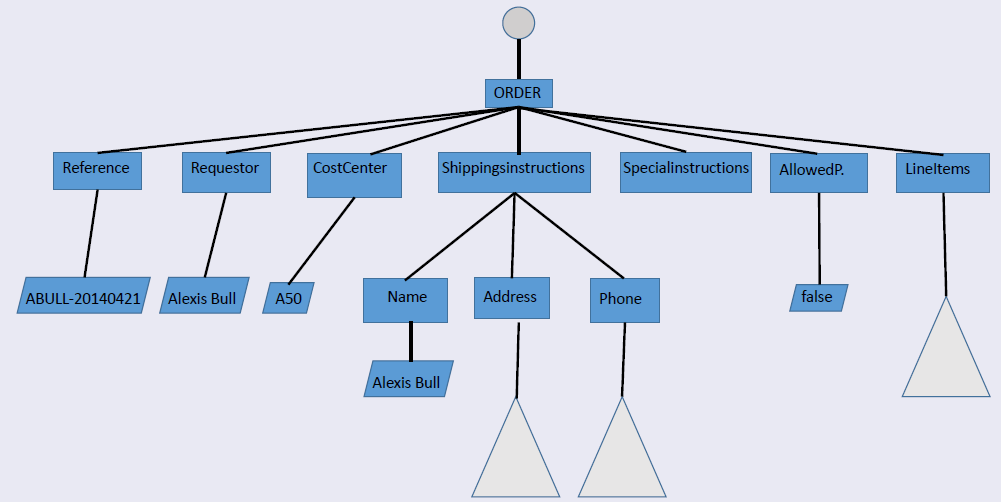
\includegraphics[scale = 0.55]{image1.png}
\end{center}
Tags are ordered, attributes not. An XML-tree is ordered (if depth-first search will reproduce the document order). The textual corresponding representation is called serialization.
It is possible document-recursion (e.g. a message in XML could contain an XML-document) but name conflicts may appear.
Definition of dbis-namespace:\\ $\mathrm{<}$xmlns:dbis=''http://.... ''$\mathrm{>}$\\
\textbf{DTD (Document Type Definition): }define attributes rules of a document (element and attributes types). A document conforms to XML syntax is \textit{well-formed, }if it is also conformed to DTD is \textit{valid.}\\
Definition of element types: \textbf{$\boldsymbol{\mathrm{<}}$!ELEMENT EName Content$\boldsymbol{\mathrm{>}}$}\\
Definition of attribute types: \textbf{$\boldsymbol{\mathrm{<}}$!ATTLIST EName Attr1 AttrType1 {\dots}.}\\
Elements types re global wrt DTD, attributes types are local.\\
\textbf{Element content: }EMPTY, ANY, (\#PCDATA) - ,{\textbar}*+?\\
\textbf{Attribute definition:}\\

\textbf{ Types: }CDATA, (Val1{\textbar}{\dots}{\textbar}Valn), ID, IDREF

\textbf{ Val: }\#REQUIRED, \#IMPLIED, val, \#FIXED val

\subsection{XPath}

XPath is a language to locate subtrees inside an XML-tree by means of location paths (sequence of steps separated by `/'). Each location is formed of an axis, a nodetest and some (opt.) predicates:

\textbf{\textit{Axis::node-test[predicate]}}\\
\begin{center}
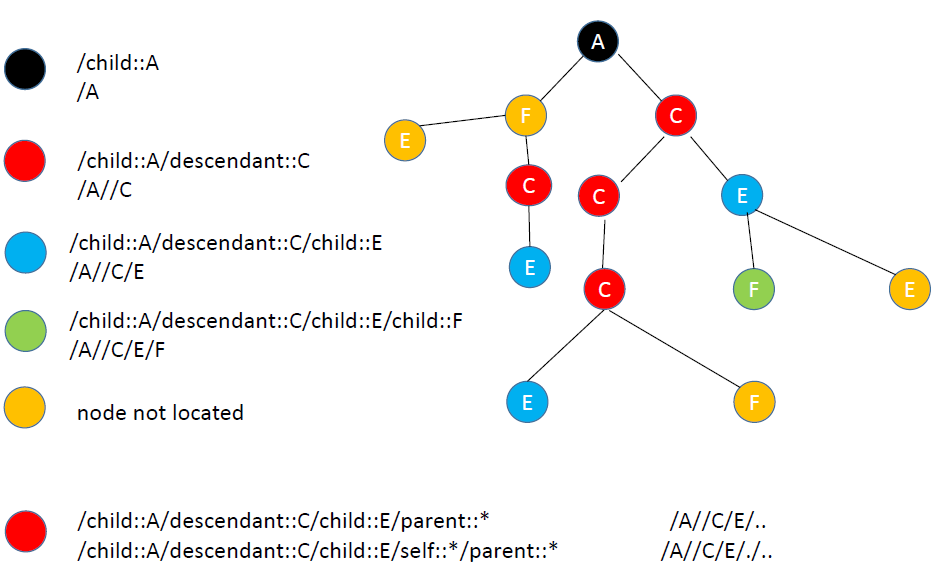
\includegraphics[scale = 0.5]{image2.png}
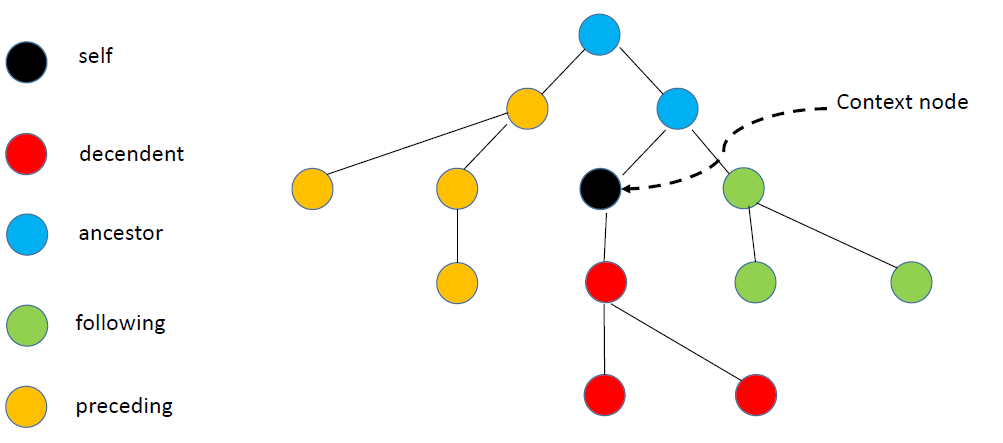
\includegraphics[scale = 0.5]{image3.png}
\end{center}
The path is evaluated relative to a respective context and locates a set of nodes. A context is given by position, size and the node. An absolute location path is the root node.
L${}_{0\ }$= $\mathrm{\{}$r$\mathrm{\}}$ -- root
L${}_{i}$(k) set of nodes determined wrt context node k.
L${}_{i\ }$= U${}_{k\ e\ Li-1}$L${}_{i}$(k).
\textbf{Node-test: }element name, *, text(), node().\\
\textbf{Predicates: }Boolean expression.\\
e.g.: /descendant::*[child::Address]\\
/child::Orders/child::Order[child::CostCenter= "A50"]/child::LineItems.\\
Context is a fact relative to a node set, is composed by: context size (cardinality), context position (its position relative to document order).

\subsection{XRel: How to store XML data physically}
\textbf{Two approaches: }Storing in  column (CLOB - Character Large OBject, type + indexing), Mapping to relational tables (Interval-based, Path-based).\\
XRel: is a Path-Based approach to storage and retrieval of XML documents using
relational databases.
\textbf{Region of an element (node test): }pair of start and end position in the XML doc.\\
\textbf{Region of an attribute: }equal to the parent node plus one.\\
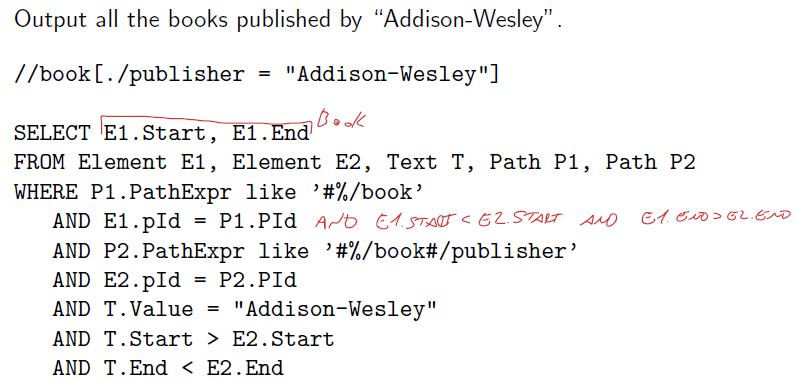
\includegraphics[scale=0.7]{4.png}\\
Use of queries with indexing.

\subsection{XQuery}
The mission of the XML Query project is to provide flexible query facilities to
extract data from real and virtual documents. Collections of XML files will be accessed like DBs.\\
XQuery is a functional language, have a declarative semantics and is strongly typed. An item is an atomic value or a node.\\
Two ways to create element node:\\\\
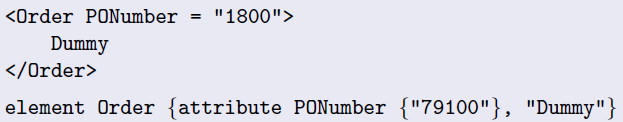
\includegraphics[scale=0.65]{5.png}
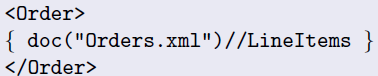
\includegraphics[scale=0.65]{6.png}\\\\
A \textbf{FLWOR-expression} is built out of \textbf{\textit{for-, let-, where-, order- and
return-}}clauses. It evaluates to a stream of tuples, where the tuples are
(variable-name, value) pairs.\\
Two main commands:\\
XMLTable: maps results of an XQuery into relational rows and columns.\\
XMLQuery: return XML-document\\
With XMLTable we refer directly to the path and use passing XMLDoc instruction. With XMLQuery we refer to doc and use RETURNING CONTENT FROM DUAL instruction.\\
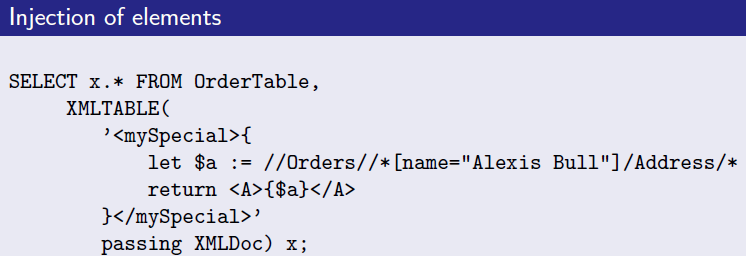
\includegraphics[scale=0.5]{7.png}
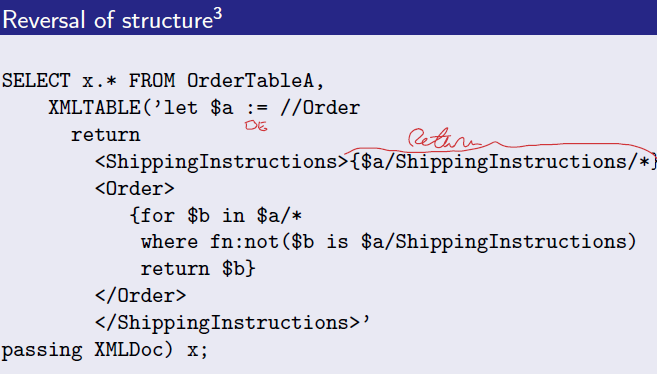
\includegraphics[scale=0.5]{8.png}\\
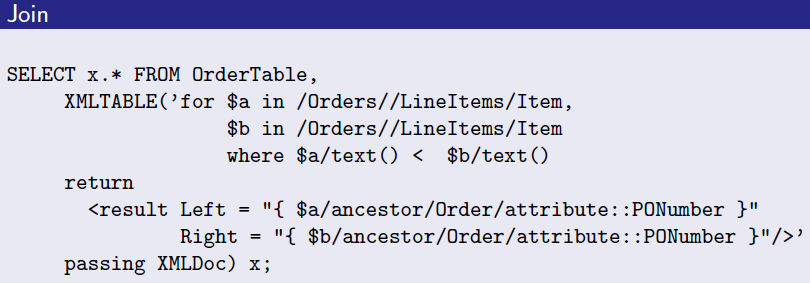
\includegraphics[scale=0.5]{9.png}\\
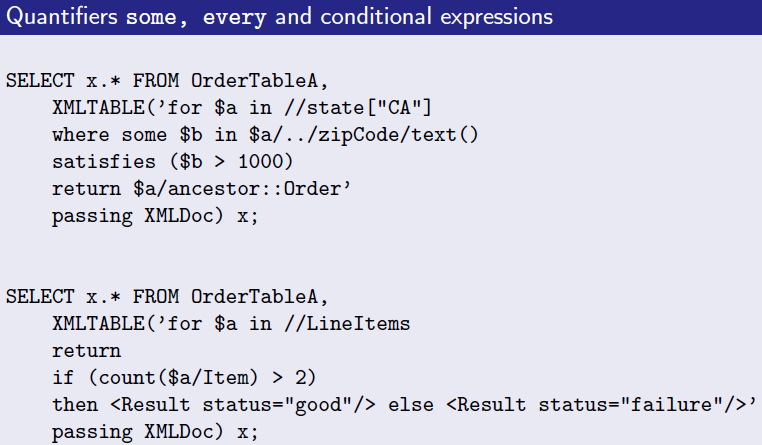
\includegraphics[scale=0.5]{10.png}
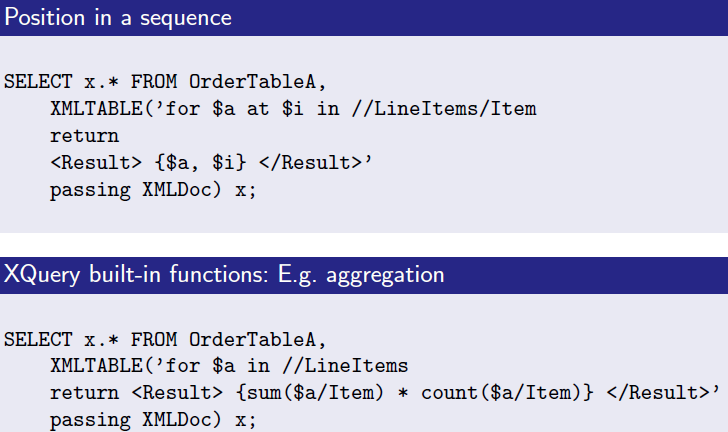
\includegraphics[scale=0.5]{11.png}\\
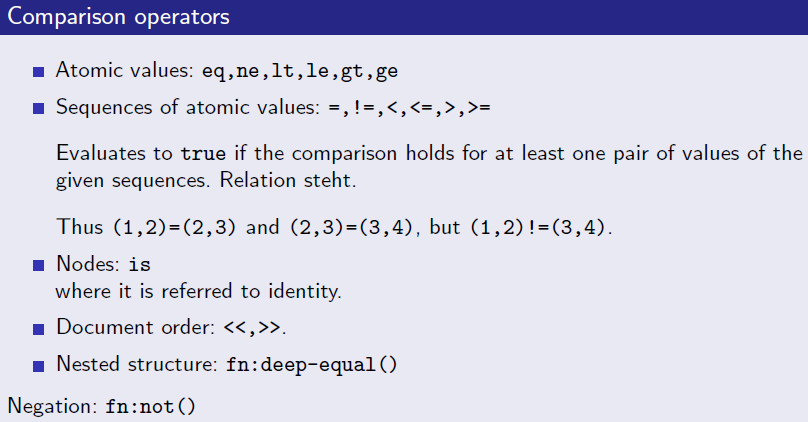
\includegraphics[scale=0.5]{12.png}\\

\section{JSON and MONGODB}

\subsection{JSON (JavaScript Object Notation)}
It is a very lightweight data exchange format based on JavaScript used for data exchange over Web.\\
It is based on two basic constructs:\\
\textbf{1. Array: }comma-separated list of things enclosed by brackets.\\
\textbf{2. Object: }comma-separated set of pairs enclosed by braces.\\\\
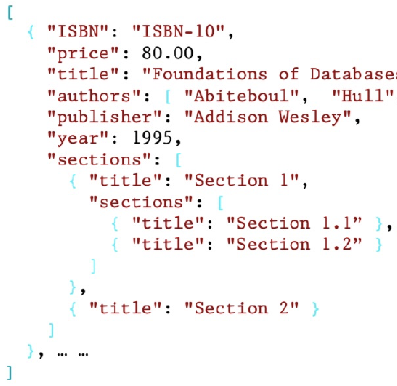
\includegraphics[scale=0.5]{18.png}\\

\subsection{MongoDB}
Document database designed for ease of development and scaling.\\
NoSQL database types:\\
\textbf{1. Key-value stores}\\
\textbf{2. Document databases:} data structure.\\
\textbf{3. Wide-column stores:} store columns of data.\\
\textbf{4. Graph stores:} store info about networks.\\
Uses JSON (BSON). MongoDB stores data records as BSON documents. BSON is a binary representation of JSON documents.\\\\
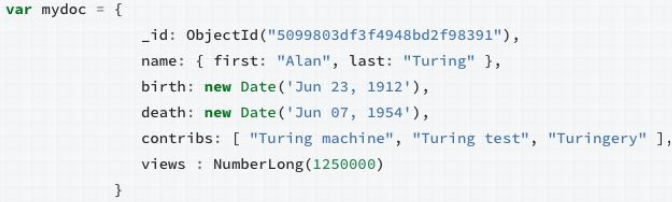
\includegraphics[scale=0.5]{19.png}\\\\
- Database = a number of collections.\\
- Collection = a list of documents.\\
- Each document stored in a collection requires a unique $\_$id
field that acts as a primary key.\\
CRUD operations: Create, Read, Update, Delete.\\
Insert commands: .insertOne(), .insertMany().\\

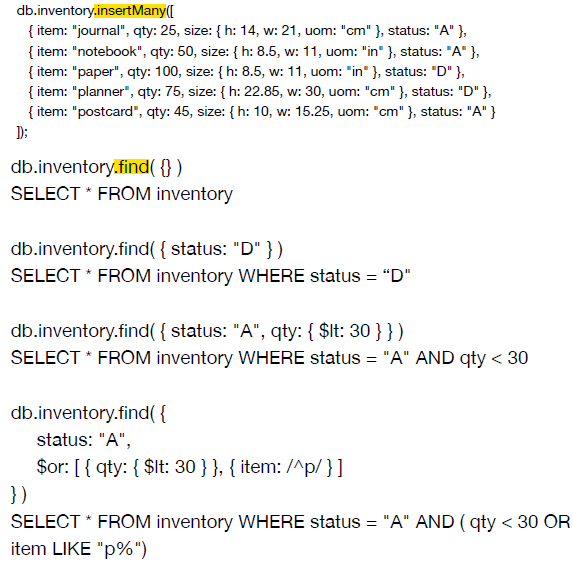
\includegraphics[scale=0.5]{20.png}
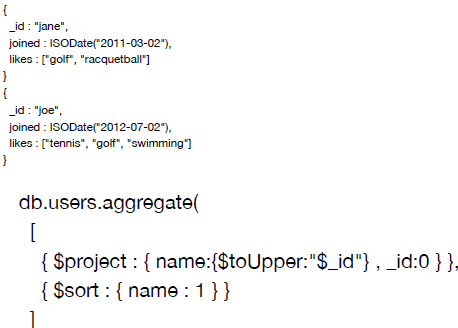
\includegraphics[scale=0.5]{21.png}\\

\begin{figure}[h!]
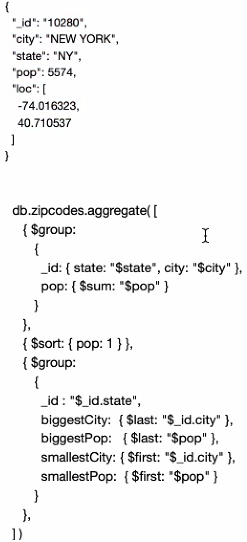
\includegraphics[scale=0.7]{13.png}
\caption{Largest and smallest cities by state.}
\end{figure}
\begin{figure}[h!]
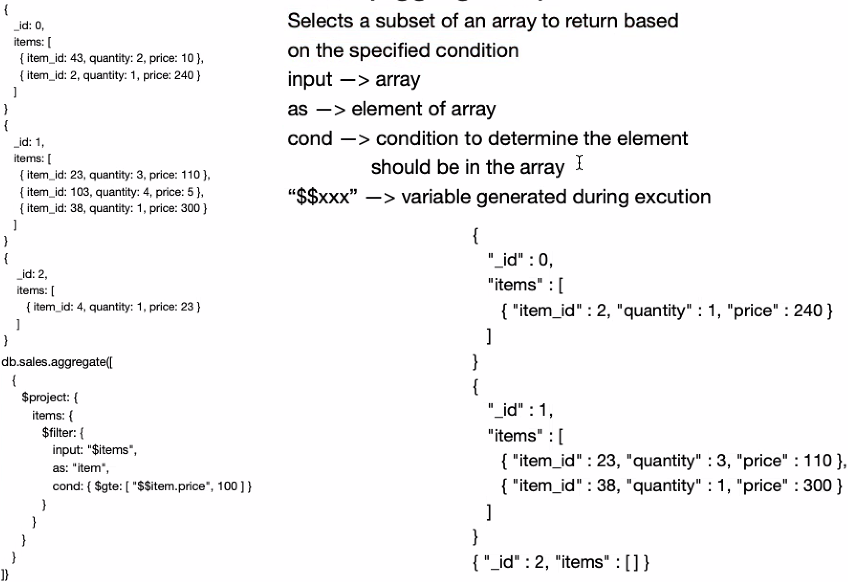
\includegraphics[scale=0.7]{14.png}
\caption{filter.}
\end{figure}

\begin{figure}[h!]
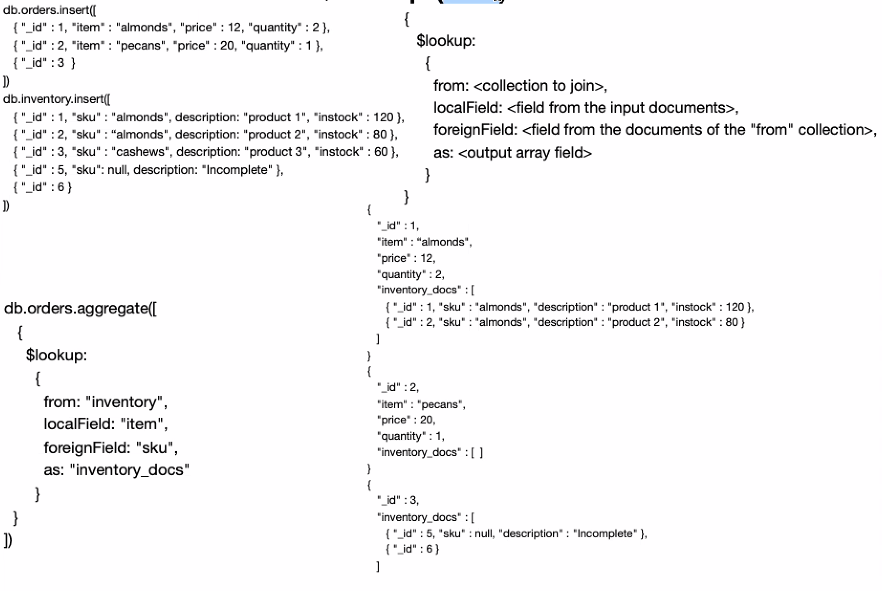
\includegraphics[scale=0.7]{15.png}
\caption{lookup(join).}
\end{figure}
\begin{figure}[h!]
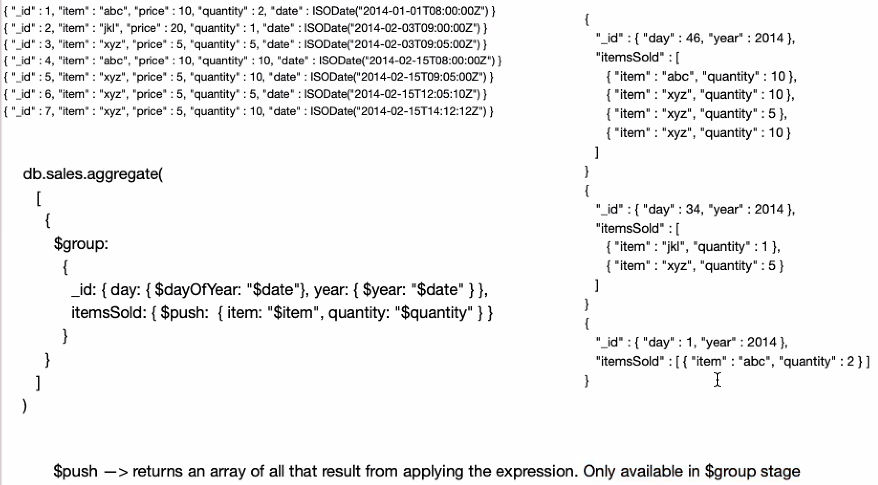
\includegraphics[scale=0.7]{16.png}
\caption{push.}
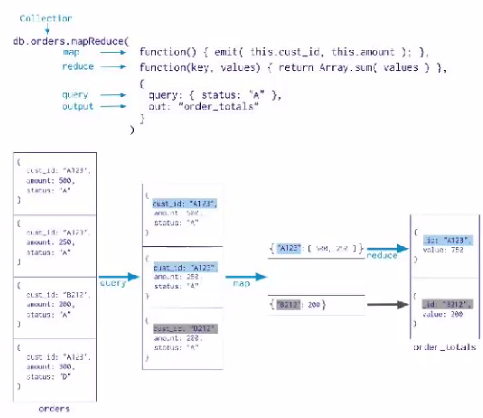
\includegraphics[scale=0.7]{17.png}
\caption{Map-reduce:Used to condense large volumes of data and emits key-value pairs. For keys with multiple values, MONGODB applies the reduce phase and then stores results in a collection.}
\end{figure}
\newpage
\section{Graph Databases}
A database that uses graph structures for storing and querying data, in a variety of domains this approach offers a more intuitive conceptualization than relational databases (e.g.: social networks).\\\\
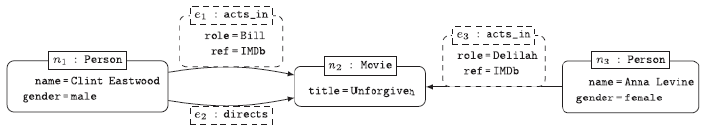
\includegraphics[scale=0.8]{22.png}[Property-graph]\\\\
\textbf{Def.:} edge-labelled graph G is a pair (V,E), E in V x Lab x V.\\
\textbf{Def.:} property graph is a tuple (v,E,$\rho$,$\lambda$,$\sigma$), where:\\
$\rho$: E $->$ (V x V), is a total function that indicate an edge from a v to another.\\
$\lambda$: V u E $->$ Lab, total function that assigns labels to vertices and edges.\\
$\sigma$: (V u E)x Prop $->$ Val, partial function with Prop a finite set of properties.\\
\subsection{Querying}
\textbf{- Pattern matching:} a match is a mapping from variables to constants such that when the mapping is applied, the result is contained in the original graph.\\
\textbf{- Navigation:} query is structured as an expression describing a topology; answers return either existance of the described structure in the original graph database, or the corresponding subgraph according to a criteria.\\
\textbf{- Set semantics:} Q(G) is defined as a set of matches; in other words, the result of evaluating Q over G cannot contain duplicate matches.\\
\textbf{- Bag semantics:} Q(G) is defined as a bag of matches; more specifically, the number of times a match appears in the result corresponds with the number of unique mappings that witness the match.\\\\
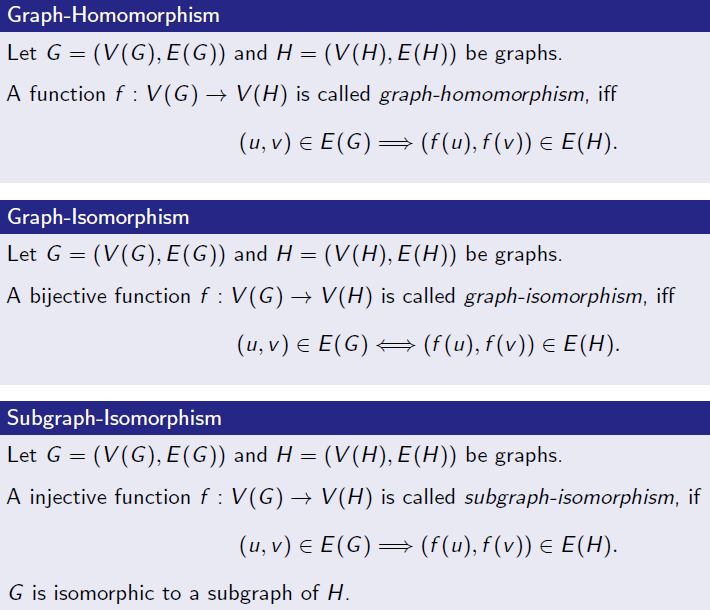
\includegraphics[scale=0.6]{23.png}\\\\
Given an edge-labelled graph G = (V, E) and a graph-pattern Q = (V', E'), a match h of Q in G = (V, E) is a mapping h : Const u Var $->$ Const such that:\\
for each constant a in Const : h(a) = a and for each edge (b, l , c) in E' : (h(b, h(l), h(c)) in E.\\
In graphs: if the image of some Q under h is contained within graph G, then h is a match.\\\\
\begin{figure}
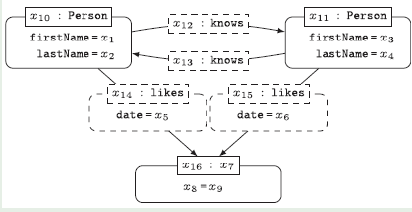
\includegraphics[scale=0.6]{24.png}
\caption= "Pattern matching query"
\end{figure}
\begin{figure}
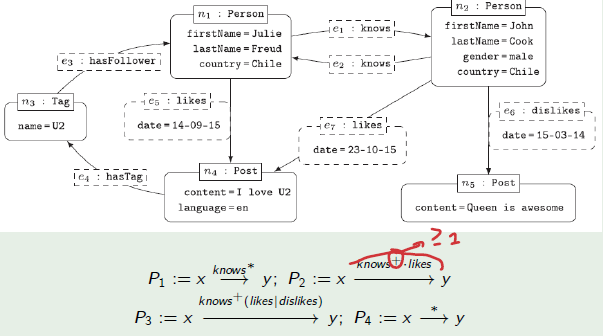
\includegraphics[scale=0.6]{25.png}
\caption= "Graph navigation query"
\end{figure}
Let a path query P = x $\alpha->$ y, where $\alpha$ is a regular expression over the set of labels, and a labelled graph G be given. The evaluation of P over G consists of all paths $\pi$ in G whose label Lab($\pi$) satisfies $\alpha$.\\\\
\begin{figure}
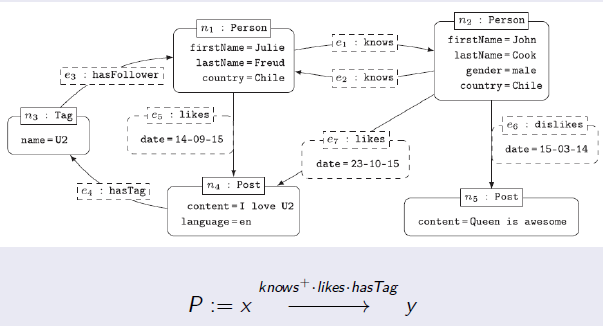
\includegraphics[scale=0.6]{26.png}
\caption= "Navigational query semantics"
\end{figure}

Can choose to return: shortest path, no-repeated-node, no-repeated-edge.

\subsection{Graph Database Query Languages}
\textbf{SPARQL } is a declarative language recommended by W3C for querying RDF ( Resource Description Framework: family of W3C specification used for conceptual description or modelling of information) graphs, a variant of edge-labelled graphs.\\\\
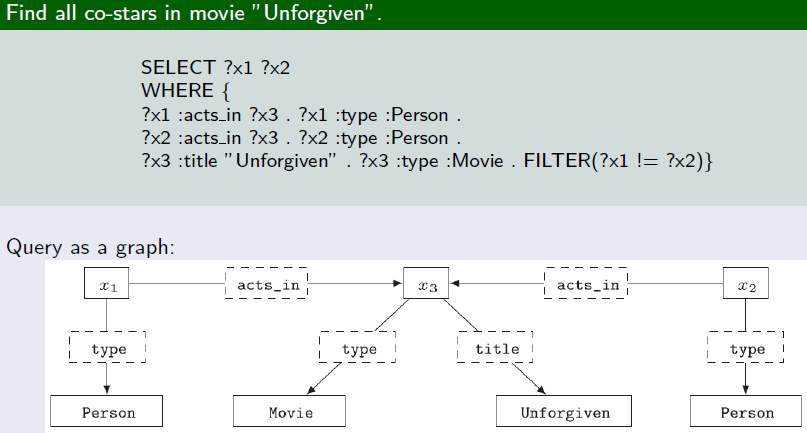
\includegraphics[scale=0.6]{27.png}\\\\
\textbf{Cypher} is the industry's most widely adopted graph database query language.\\\\
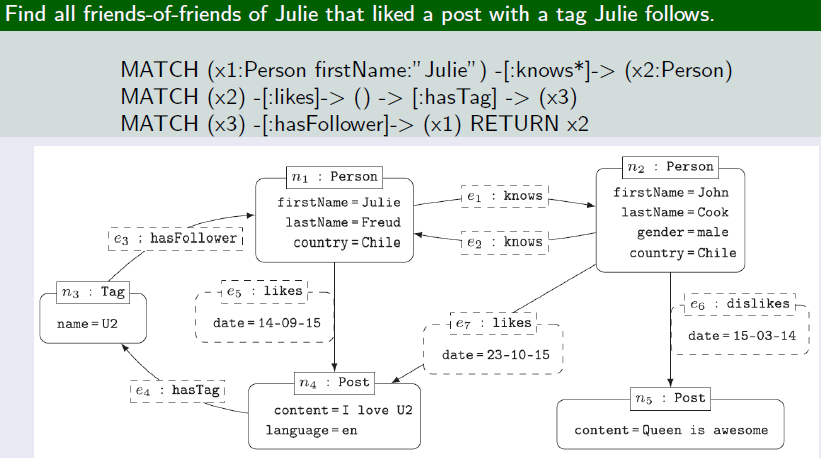
\includegraphics[scale=0.6]{28.png}\\\\
\textbf{Gremlin }is the query language of the Apache Tinker-Pop3 graph Framework.
It feels more like a programming language interface. Likewise, its focus is on navigational queries rather than matching patterns.\\\\
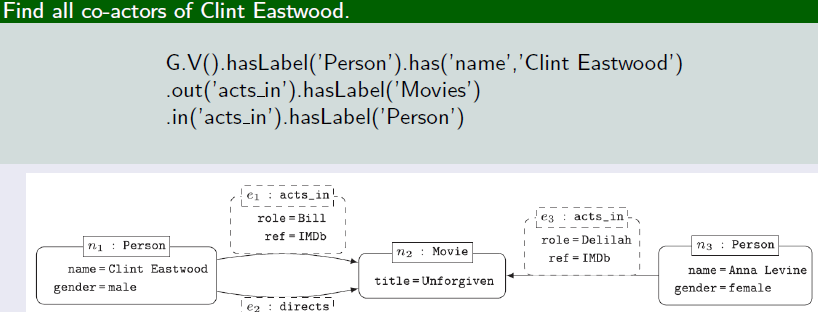
\includegraphics[scale=0.6]{29.png}\\\\
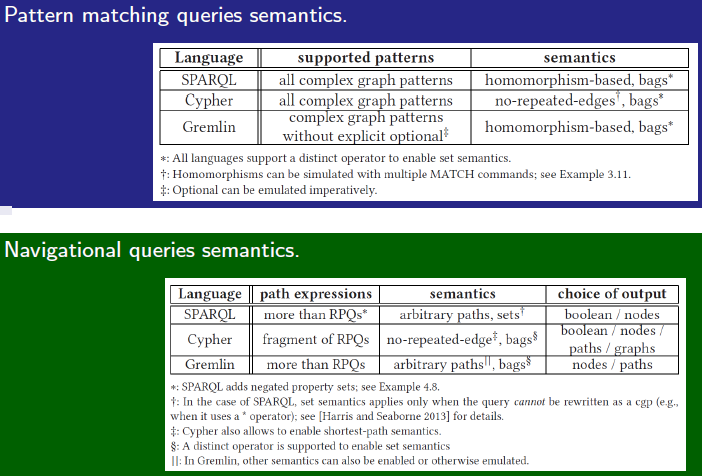
\includegraphics[scale=0.6]{30.png}\\\\


\section{Beyond Relatioknal Database Systems: Column, NoSQL, Graph-DB}
\subsection{Column-Stores}
Column-stores is a type of storing based on column-wise. Why? Buffer management (only columns needed get), data locality (value aggregations), compression (values are same type), insertion and materialization. Why not? Tuple insertion and reconstruction.\\
\textbf{- Data model: }$\tau$ = dom | <A1: $\tau$[*|?],....,An: $\tau$[*|?]>\\
\textbf{- Repetition level:} denotes at which level in the path the last repetition occured. Useful to understand when to start a new list and where. (R = 0 means new record)\\
\textbf{- Definition level:} How many nested fields in a path that could be undefined are present.\\\\
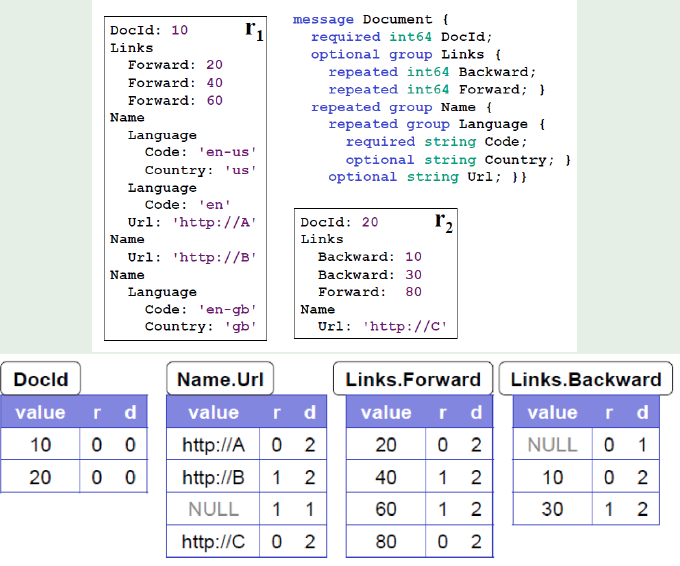
\includegraphics[scale=0.6]{31.png}\\\\

\subsection{NoSQL (Not Only SQL) Database System}
NoSQL database system may be non-relational, support non-standard query languages, support schema evolution and independance, support data distribution with possibly a weaker form of consistency.\\\\
\textbf{- Key-value Store} \\
Prototype of a schema-less database: arbitrary key-value pairs can be stored and
retrieved; simple, but quick. \textbf{Adv.: }data easily distributed. \textbf{Disadv.: }No query language.\\\\
\textbf{Wide-column Store}\\
Data is stored in tables (not normalized), where records have the ability to hold very large numbers of dynamic columns. Concept of column families, multidimensional keys etc.\\\\
\textbf{- RDF-storage by Relational Databases approaches:}\\
\textbf{1. Triple table\\\\}
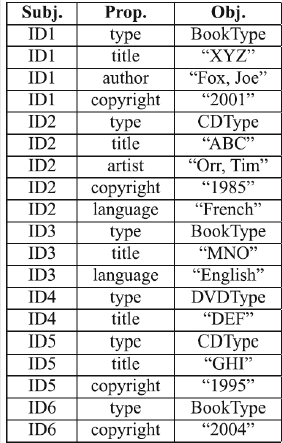
\includegraphics[scale=0.6]{32.png}\\\\
Advantage: Simplicity. Problems: Multi-way self-joins may result, which, when not selective, are very
expensive.\\\\
\textbf{2. Property table\\\\}
\textbf{Advantage:} Subject-Subject self-joins are reduced; attribute-typing possible. \textbf{Problems:} Queries with unspecied property values are problematic. NULL-values may yield sparse tables. What to do with multi-valued attributes?
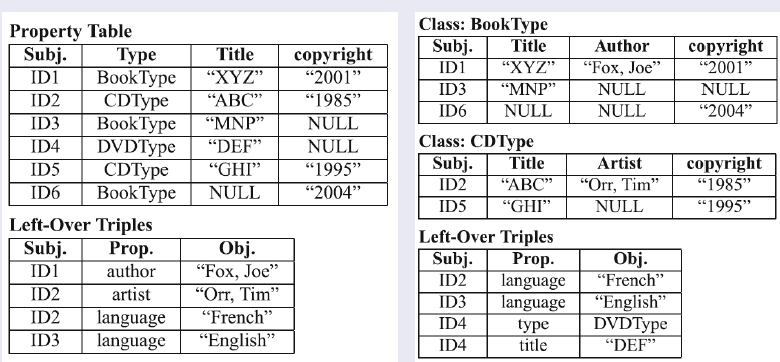
\includegraphics[scale=0.6]{33.png}\\\\
\textbf{3. Vertically partitioned approach}\\\\
\textbf{Advantages:} Support for multi-valued attributes. Support for heterogenous records. Reduced I/O-costs: only that what indeed is needed will be accessed. No property-clustering required. \textbf{Problems: }Increased number of joins. Queries with unspecied properties. Inserts.\\
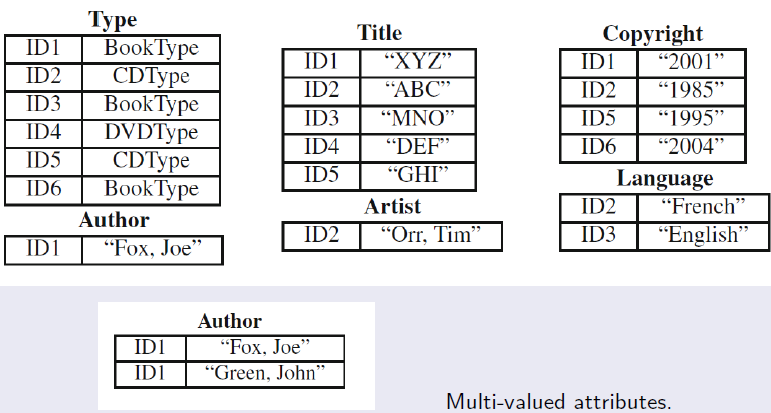
\includegraphics[scale=0.6]{34.png}\\

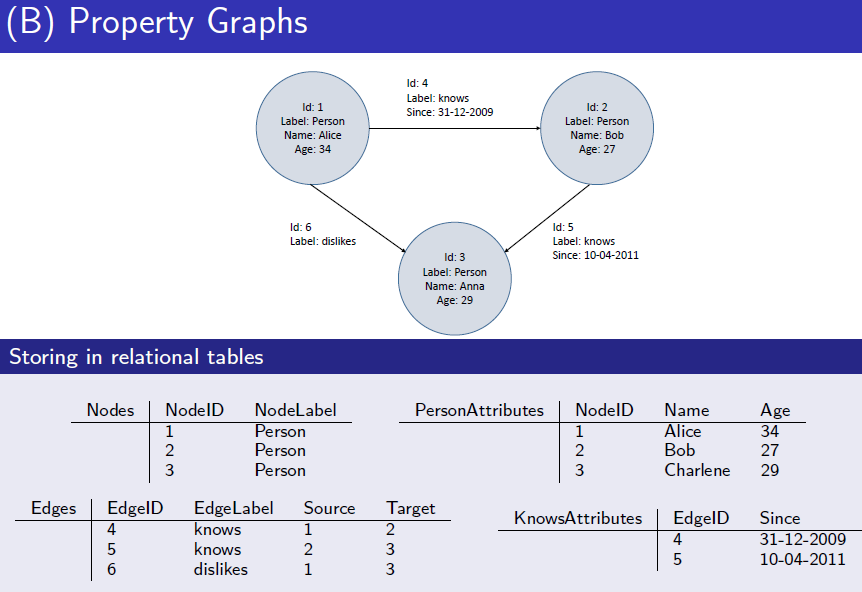
\includegraphics[scale=0.6]{35.png}\\

\section{Distributed Processing with Computer Clusters}
Big Data is just Data but bigger, often characterized by the 3 (or 4) V$'$s:\\
• Volume\\
• Variety\\
• Velocity\\
• (Veracity)\\\\
Distributed processing of Big Data requires non-standard programming models. One of the most popular frameworks is \textbf{MapReduce}: algorithms expressed as a sequence of Map() and Reduce() functions.\\\\
\subsection{MapReduce}
\textbf{- Ideas behind MapRedure: }scale out, not up. Assume failures are common (but few). Take advantage of data locality and avoid to transfer large datasets. Process data sequentially and avoid random access. Hide system-level details (so devs can focus not on dealing with DS). Seamless scalability (transparency).\\
\textbf{- DFS (Distributed File System): }Data is split into equally sized blocks and stored distributed, fault tolerance thanks to replication, write-once$/$read-many.\\
\subsection{Clusters}
Why? Data mining on a single server not enough. Cluster Architecture:\\\\
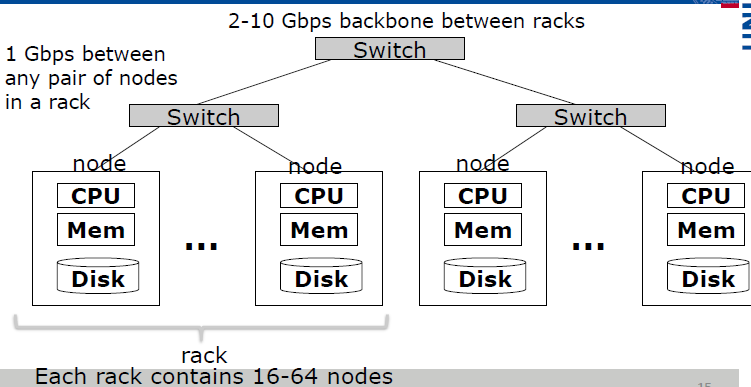
\includegraphics[scale=0.6]{36.png}\\\\
\textbf{- Google File System (GFS)}\\\\
\begin{figure}[h!]
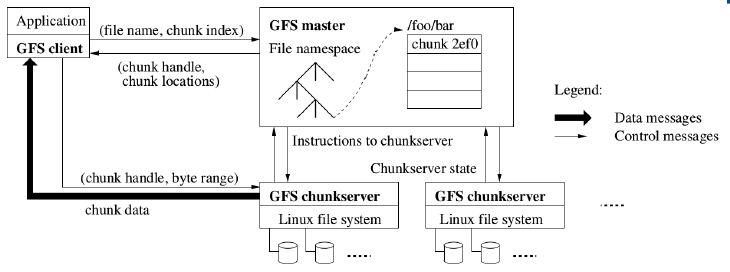
\includegraphics[scale=0.6]{37.png}
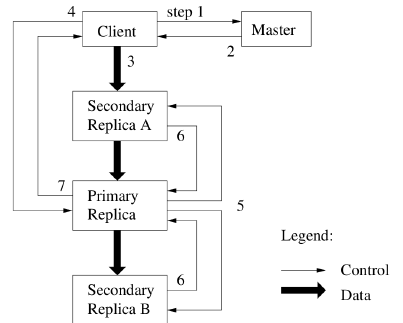
\includegraphics[scale=0.6]{38.png}
\end{figure}
\subsubsection{Basic Components of a DFS: }
\begin{itemize}
\item \textbf{1. Chunk Servers} File is split into contiguous replicated chunks (64-256 MB) in different racks.
\item \textbf{2. Master Node} Stores metadata and might be replicated.
\item \textbf{3. Client library for file access} Talks to master to find chunk servers and connect directly to them.
\end{itemize}
Back in the MapReduce topic, Approach: target problem needs to be parallelizable:\\problem gets split into smaller problems (Map), then they are solved in a parallel way, finally, they get synthesized into a solution of the original problem (Reduce step).\\\\
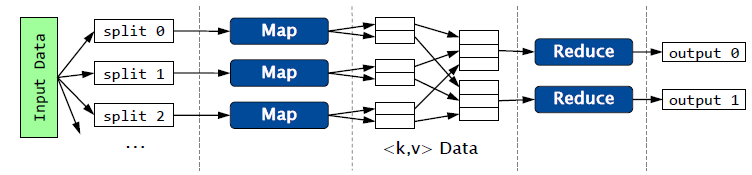
\includegraphics[scale=0.6]{39.png}\\\\
\textbf{- Distributed Execution}\\\\
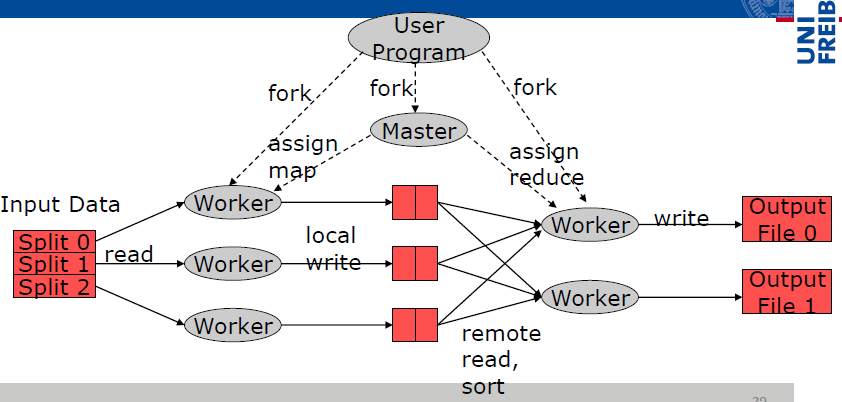
\includegraphics[scale=0.6]{40.png}\\\\
Intermediate results are stored on local file system of map- and reduce-workers. Output is often input to another MapReduce task.\\\\
map(k,v) $->$ list(k1,v1)\\
reduce(k1, list(v1)) $->$ v2\\\\
To coordinate the work it is used a \textbf{Master} as "central unit" for coordination (it also check for failures):\\
\begin{itemize}
\item \textbf{-}Idle tasks get scheduled as workers become available, 
\item \textbf{-}When a map task completes, it sends the master the location and sizes of its R intermediate files, one for each reducer.
\item \textbf{-}Master pushes this information to reducers.
\end{itemize} 
There are different types of failures:\\
\begin{itemize}
\item \textbf{Map worker failure: }Map tasks completed or in-progress at worker are reset to idle; Reduce workers are notified when task is rescheduled on another worker.
\item \textbf{Reduce worker failure: }only in-progress tasks are reset to idle.
\item \textbf{Master failure: }MapReduce task is aborted and client is notified.
\end{itemize}
Make M (map tasks) and R (reduce tasks) much larger than the number of nodes in cluster (usually R$<$M).\\
Often it can happen that many pairs are combined for the same key, solution: pre-aggregating at mapper: combine (k1, list(v1)) $->$ v2.  Works only if reduce function is commutative and associative.\\\\
\textbf{- Partition function: }Inputs to map tasks are created by contiguous splits of input file. For reduce, we need to ensure that records with the same
intermediate key end up at the same worker. System uses a default partition function e.g., hash(key) mod R. Sometimes useful to override.\\

\section{Spark}
Open-source, distributed, general-purpose cluster computing framework. For processing large volumes of data, both batch processing and streaming. \\
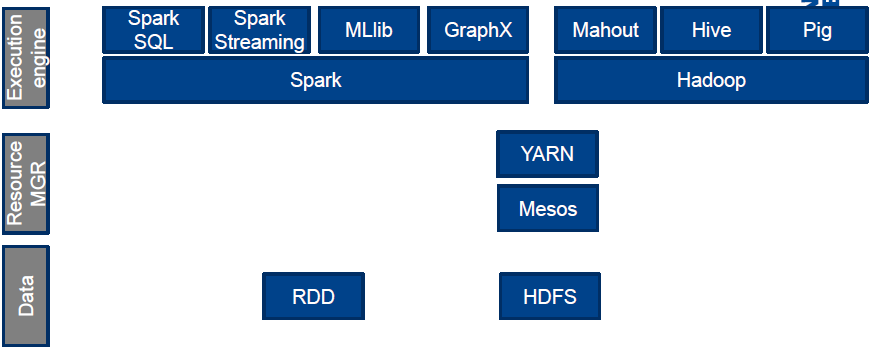
\includegraphics[scale=0.6]{41.png}\\\\
More general functional programming model than MapReduce: Transformations and actions. In spark Data is organized in RDDs \textbf{(Resilient Distributed Datasets)}, properties: \textit{immutable, resilient, distributed.} Transformation are parallel and construct a new RDD, Action are just performed on RDD's elements. Job is broke into tasks by the \textbf{driver}. \textbf{Spark context:} sets up internal services and establishes a connection to a Spark execution environment.\\\\
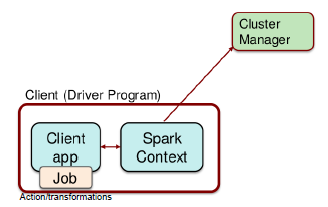
\includegraphics[scale=0.6]{42.png}
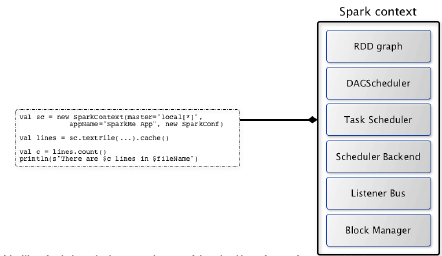
\includegraphics[scale=0.6]{43.png}\\\\
The \textbf{worker node} has one or more executors, talks with cluster manager, receive tasks. Data, in general, is organized in RDDs, created by:\\
\begin{itemize}
\item Create from any file stored in HDFS or other supported storage.
\item Streaming sources (via Spark Streaming).
\item An RDD can be the output of a Spark transformation function.
\end{itemize}
In Spark: \textbf{Directed Acyclic Graph (DAG) }created and submitted to \textbf{DAG scheduler}, more efficienct than \textbf{MapReduce}, since DAG optimizer rearranges the order of the operators and since data is cached.
\subsection{Transformations}
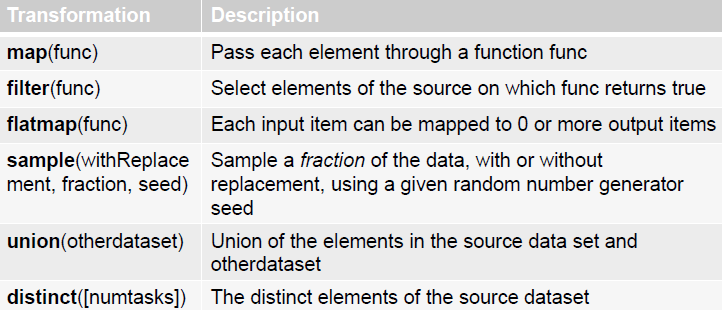
\includegraphics[scale=0.6]{44.png}
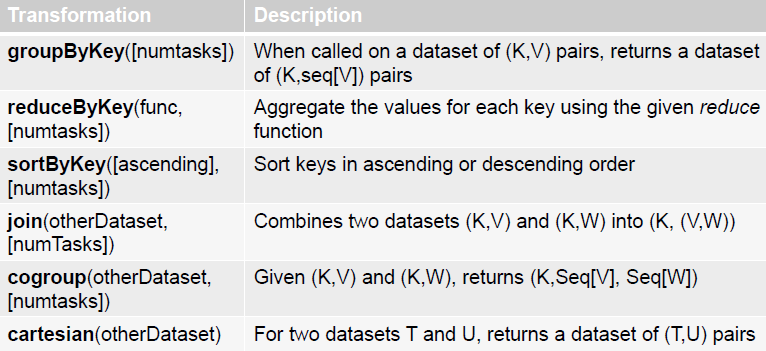
\includegraphics[scale=0.6]{45.png}\\\\
\subsection{Actions}

\includegraphics[scale=0.6]{46.png}
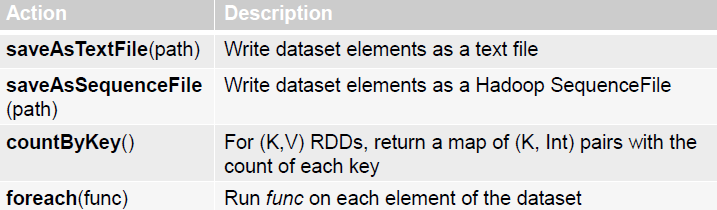
\includegraphics[scale=0.6]{47.png}\\\\
\subsection{Data storage}
Spark does not care how source data is stored, RDD fault tolerance: RDDs track the sequence of transformations used to create them, enables recomputing of lost data.\\
\textbf{- Example:}\\\\
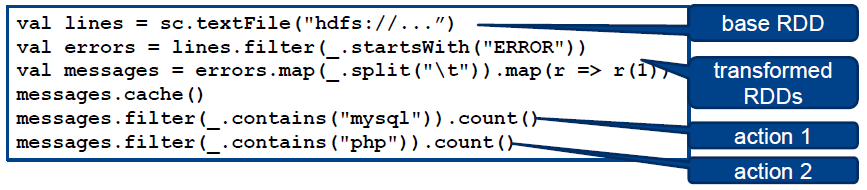
\includegraphics[scale=0.6]{48.png}\\\\
\subsection{Spark Streaming}
Differently from MapReduce etc, it enables processing of live data streams.\\\\
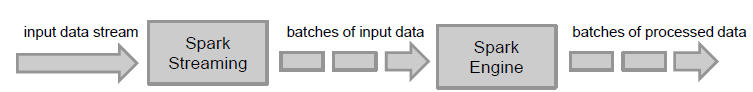
\includegraphics[scale=0.6]{49.png}\\
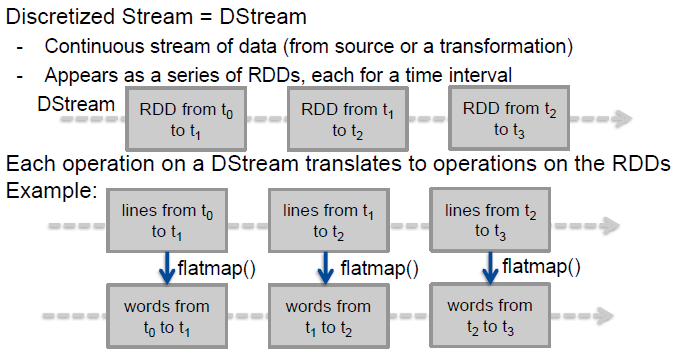
\includegraphics[scale=0.6]{50.png}\\\\
\subsection{Dataframe in Spark}
Handle structured data in a table-like representation (with column names/types) and translate SQL code and domain-specific language (DSL) expressions into optimized low-level RDD operations.\\\\
\includegraphics[scale=0.6]{51.png}\\\\
\subsubsection{Create Dataframe}
\begin{itemize}
\item Converting existing RDDs
\textbf{a)} Using RDDs containing row data as tuples\\\\
\includegraphics[scale=0.6]{52.png}\\\\
\textbf{b)} Using case classes\\\\
In columns all strings so far $=>$ Introduce data types via case classes.\\
\textbf{Steps: }\textbf{(a)} define case class, \textbf{(b)} map each row in RDD to case class, \textbf{(c)} use toDF method. For better conversion (of different data types, i.e., to not only have strings), define class and methods.\\
\textbf{c)} Specifying a schema\\
Use SparkSession’s createDataFrame method (needed: objects of type Row and a StructuredType (=schema)). Actual transformation (now Row, not Post type.\\\\
\textbf{How to use DataFrame API}\\\\
\includegraphics[scale=0.6]{53.png}
\includegraphics[scale=0.6]{54.png}\\\\
\item Running SQL queries
SQL functions are available through: \textbf{Datframe API} and \textbf{SQL expressions} of these types:\\
\begin{itemize}
\item \textit{Scalar functions: }return single value for each row. e.g. \textbf{Math calulations or String operations}
\item \textit{Aggregate functions: }return single value for a group of rows. 
\item \textit{Window functions: }return several values for a group of rows. e.g. to make selects and joins simpler. import \textit{expresisons.Window}
\item \textit{User-defined functions: }include custom scalar or aggregate functions.
\end{itemize}
\textbf{- Using SQL commands in Spark: }\\
Commands get translated into DataFrames. Spark supports Spark's SQL dialect and Hive Query Language (HQL). One can store DataFrames as tables in a table catalogue (either temporary or permanently).\\
\textbf{- Example: }\\
\textit{spark-sql> select substring(title, 0, 70) from posts where\\
postTypeId = 1 order by creationDate desc limit 3;}
\item Loading external data

\end{itemize}

\section{Graph Query Language Semantics}
Most widely used query languages in practice but offer significant differences:\\
- SPARQL operates over RDF graphs, i.e. edge-labelled graphs;
- Cypher is designed to operate over property graphs;
- Gremlin is more imperative in nature than the other two, geared more towards graph traversal than graph pattern matching.\\
\includegraphics[scale=0.6]{55.png}\\\\
\subsection{Conjuctive Queries}
A \textit{conjunctive Query }Q over a database schema R is given as:\\
\begin{equation}
ans(U) <- R_1(U_1),...,R_n(U_n)
\end{equation}
\begin{itemize}
\item $R_i$ relation name in R.
\item U and $U_i$ vectors of variables and constants.
\item any variable in U is also in $U_i$
\item Left to $<-$ is the head, right the body.
\end{itemize}
\includegraphics[scale=0.6]{56.png}\\\\
The set of answers Q w.r.t. an instance I of the given relations is denoted Q(I).\\If there is a substitution (match, mapping) $\sigma$ from the variables in U1,...,Un. to the constants in dom, such that $\sigma$(R1(U1)),...,(Rn(Un)) in I, then by applying the same substitution $\sigma$ to U, we say that $\sigma$(ans(U )) is an answer in Q(I).\\
Substitutions are functions - a constant is mapped into itself.\\
\textbf{-Definitions: }\\\\
\includegraphics[scale=0.6]{57.png}\\
\includegraphics[scale=0.5]{58.png}
\includegraphics[scale=0.5]{59.png}\\
\includegraphics[scale=0.6]{60.png}\\\\
\textbf{- Substitution: }\\
A substitution $\theta$ over a set of variables V is a mapping from V to V U dom,
where dom a corresponding domain. We extend $\theta$ to constants a in dom and relation names R in R, where $\theta$(a) = a, resp. $\theta$(R) = R. Differently to a match, variables may be renamed, i.e. mapped to variables.\\
Substitution $\theta$ is called containment mapping from Q2 to Q1, if Q2 can be
transformed by means of $\theta$ to become part of Q1:\\
\begin{itemize}
\item $\theta$(ans(V))=ans(U)
\item for i = 1,...,m there exists a j in {1,...,n}, such that $\theta$(Si(Vi)) = Rj(Uj).
\end{itemize}
\includegraphics[scale=0.6]{61.png}\\
\includegraphics[scale=0.6]{62.png}\\\\
\includegraphics[scale=0.6]{63.png}\\
\includegraphics[scale=0.6]{64.png}\\\\
\textbf{- Example: }\\
\includegraphics[scale=0.6]{65.png}\\\\
\includegraphics[scale=0.6]{66.png}\\
\includegraphics[scale=0.6]{67.png}\\
\includegraphics[scale=0.6]{68.png}
\subsection{Minimization of Conjunctive Queries}
A query Q' is a subquery of a query Q, if the body of Q' is a subset of the body of Q.\\
\includegraphics[scale=0.6]{69.png} \\\\
\includegraphics[scale=0.6]{70.png} \\\\
\textbf{Query minimization is NP-hard.}\\
\includegraphics[scale=0.6]{71.png} \\\\
\includegraphics[scale=0.6]{72.png} \\\\

\section{Acyclic Conjuctive Queries}
\begin{center}
    A conjunctive query Q is \textbf{acyclic} if it has a join tree.\\
    Let $Q(x) = R_1(z_1),...,R_n(z_n)$ be a CQ. A \textbf{join tree} T = (V,E) is a tree where:\\
    - $V = {R_1(z_1),...,R_n(z_n)}$, i.e. V is the set of atoms in Q \\
    - \textbf{E} satisfies for all variables z of Q:\\
    ${R_j(z_j) \in V|z occurs in R_j(z_j)}$ induces a connected subtree in T.
\end{center}
\includegraphics[scale=0.4]{73.png}\\\\
 \subsection{Finding Join Trees}
Existence of a join tree can be efficiently decided and computed (if one exists). Test for acyclicity, easy to identify a quesry with a hypergraph. \textbf{Def: }Atom R(z) is empty if $|z|=0$ and Atom $R_1(z_1)$ is contained in atom $R_2(z_2) if z_1 \subseteq z_2$.\\
$\longrightarrow$ \textbf{GYO-reduction}
Let $Q(x) = R_1(z_1),...,Rn(z_n)$ be a CQ. Apply the following rules until possible:\\
\textit{GYO-reduction: }Eliminate variables containd in at least one atom and atoms empty or contained in another atom.\\
\textit{GYO'-reduction: }Eliminate atoms that share no variables with other atoms and atoms R if there exists a witness R': each variable in R either appears in R only, or also in R'.\\
\begin{center}
GYO'(Q) = \empty iff GYO(Q) = \empty\\
GYO’(Q) = \empty iff Q has a join tree (iff Q is acyclic)
\end{center}
\begin{center}
    See the proof if needed.
\end{center}
\subsection{Deciding ACQs Efficiently (Yannakakis)}
\textit{Algorithm by Yannakis}\\\\
Let T = (V,E) be a join tree of a query Q. Given database instance D, decide Q(D) = \empty as follows:\\
\begin{itemize}
\item \textbf{1. }Assign to each $R_j(z_j)\in V$ the corresponding relation $R_j^D$ of D
\item \textbf{2. }In a bottom up traversal of T: compute semijoins of $R_j^D$
\item \textbf{3. }If the resulting relation at root node is \textbf{empty} (then Q(D) = \empty), \textbf{nonempty} (then Q(D)$\neq$)\\
\end{itemize}
\textbf{Theorem: }For ACQs Q: \textbf{Deciding} Q(D) = \empty is feasible in polynomial time, \textbf{Computing} Q(D) can be done in output polynomial time.\\\\
\includegraphics[scale=0.6]{74.png}\\\\
\subsection{Yannakakis Enumeration Algorithm: }
\begin{quote}
    Theorem: Let Q be an acyclic conjuntive query. Given some database instance D, Q(D) can be computed in output polynomial time, i.e., in time $O((||D||+||Q(D)||)^k)$.\\
    \textit{Algorithm: }\\
    \begin{itemize}
        \item \textbf{1. }$1^{st}$ bottom-up traversal: semijoins as before (upwards propagation)
        \item \textbf{2. }top-down traversal: "reverse" semijoins (downwards propagation)
        \item \textbf{3. }$2^{nd}$ bottom-up traversal: compute solutions using joins.
    \end{itemize}
    See proof if needed.
\end{quote}
\textbf{- Example: }\\
\includegraphics[scale=0.3]{75.png}
\includegraphics[scale=0.3]{76.png}
\newpage
\section{Datalog}
Query: MATCH (X:Airport Location:”FFT”) -[:Flight*]$->$ (Y:Airport) RETURN Y\\
Queries are expressed as rules (akin to triggers in SQL). Fully logic-based query language.\\
Queries are expressed as rules. A rule is an implication of the form: $H(U) \leftarrow L_1,...,L_n$. $L_i$ are literals, H(U) is an atom. Literals in the body are called subgoals. A set of rules is called program.\\
\begin{itemize}
\item Which destinations are reachable from Frankfurt (FFT) with direct flight connection?\\
FDest(X) $\leftarrow$ Flight($\_,'FFT',X,\_,\_$)
\item Which destinations can be reached from Frankfurt (FFT) when starting at 9:00 and changing the plane at most once?\\
FDest9am(X) $\leftarrow$ Flight($\_,'FFT',X,'9:00',\_$)\\
FDest9am(Y) $\leftarrow$ Flight($\_,'FFT',X,'9:00',\_), Flight(\_,X,Y,\_,\_$)
\item Which destinations can be reached from Frankfurt (FFT)? Recursion!\\
DestRec(X) $\leftarrow$ Flight($\_,'FFT',X,\_,\_$)\\
DestRec(Y) $\leftarrow$ DestRec(X), Flight($\_,X,Y,\_,\_$)
\item Which destinations can be reached from Frankfurt (FFT) taking only Lufthansa (LH)
flights?\\
LHDestRec(X) $\leftarrow$ Flight($'LH','FFT',X,\_,\_$)\\
LHDestRec(Y) $\leftarrow$ LHDestRec(X), Flight($'LH',X,Y,\_,\_$)
\item All destinations that can be reached from Frankfurt except those for which a
Lufthansa-only (!) connection exists. Negation!\\
Destination(X) $\leftarrow$ DestRec(X), $\neg$ LHDestRect(X)
\end{itemize}
\textbf{- Framework}\\\\
\includegraphics[width=0.4\textwidth]{77.png}\\
If the body is empty, the rule is called \textit{fact}, Relation symbols that appear solely on the body of rules are called \textit{extensional}; the remaining relational symbols are called \textit{intensional}. A set of rules $\rho$ is called program $\Pi$. The dependancy graph is a directed, labeled digraph containing two types of edges: if contains a negative literal $\rightarrow$ negative edge, otherwise, positive edge. We call a program recursive, if its dependency graph has a cycle.\\
\textbf{- Definition: Active Domain of an Instance} adom(I) is the set of all constants appearing in I.\\
\textbf{- Definition: Active Domain of a Datalog program} adom($\Pi$,I) is the set of all constants appearing in $\Pi$ ad I.\\
A rule is called \textbf{safe }if every variable appears in a positive literal in its \textbf{body}.\\
\textbf{Lemma: }Let $\Pi$ be a Datalog program. If every rule of $\Pi$ is safe and $I_E$ is finite, then the output $I_A$ of $\Pi$ is finite.
\begin{itemize}
\item \textbf{Example: Safe Datalog Program}\\
DestRec(X) $\leftarrow$ Flight($\_,‘FFT’,X,\_,\_$)\\
DestRec(Y) $\leftarrow$ DestRec(X), Flight($\_,X,Y,\_,\_)$
\item \textbf{Example: Non-safe Datalog Program}\\
Goal(X) $\leftarrow $Flight($\_,‘FFT’,Y,\_,\_)$\\
X doesn't occure in a positive literal in the body.
\item \textbf{Example: Non-safe Datalog Program}\\
Goal(X) $\leftarrow$ $\neg$ Flight($\_,‘FFT’,X,\_,\_)$
\end{itemize}
\textbf{Datalog+} Positive datalog\\
\textbf{Datalog$\neg$} Positive and Negative datalog\\
\textbf{Datalog$\neg\neg$} negative also in head\\
\textbf{Stratified Datalog$\neg$} defined later\\
\textbf{NR-Datalog$\neg$} Non-recursive datalog with negation\\
\textbf{$Datalog^{wff}$ , $Datalog^{stable}$}: Negated datalog beyond stratification\\\\
\includegraphics[scale=0.3]{78.png}\\
\includegraphics[scale=0.3]{79.png}\\\\
Given a $Datalog^+$ program $\Pi$, the naive evaluation algorithm always terminates.\\\\
\includegraphics[scale=0.3]{80.png}
\includegraphics[scale=0.3]{81.png}\\\\
\textbf{- Semi-naive: }To derive in round i+1 a new fact, we have to use a fact derived in the last round as a new fact.\\\\
\includegraphics[scale=0.3]{82.png}\\\\

\subsection{Semantics}
Two possible views:
\begin{itemize}
\item \textbf{Rules are First-order Logic formulas} $\rightarrow$ model-theoretic or proof-theoretic.
\item \textbf{Rules are operational rules} $\rightarrow$ Fixpoint semantics
\end{itemize}

\subsubsection{Model-theoretic Semantics}
I can be understood as a set of (database) facts of the form : ${R(a_1,...,a_n)|R \in R,(a_1,...,a_n)\in I(R)}$.\\
Let $\rho$ be a rule: $\rho=H \leftarrow G_1,...,G_k$ and I an instance, then:\\
\begin{quote}
I satisfies $\rho$, if for each assignment v of the variables in $\rho$: $v(G_1),...,v(G_k)\in I \rightarrow v(H)\in I$.\\
I satisfies $\Pi$ iff it satisfies every rule $\rho$ from $\Pi$
\end{quote}
\includegraphics[scale=0.3]{83.png}\\
\textbf{- Preliminars:}\\\\
Let $\Pi$ be a Datalog program, let R be a database schema that contains exactly the relational symbols appearing in $\Pi^2$ and let edb($\Pi$) (idb($\Pi$)) denote the set of extensional
(intensional) relational symbols of $\Pi$. The input for $\Pi$ is an instance over edb($\Pi$).
A model of $\Pi$ is an instance over R, i.e. edb($\Pi$) $\cup$ idb($\Pi$), that satisfies $\Pi$.\\\\
\textbf{- Def: Model-theoretic Semantics: }The model-theoretic semantics of $\Pi$ w.r.t. to input I, denoted as $\Pi$(I), is the minimal model of $\Pi$ containing the input I.

\subsubsection{Fixpoint Semantics}
\includegraphics[scale=0.3]{84.png}\\
\includegraphics[scale=0.3]{85.png}\\
\includegraphics[scale=0.3]{86.png}\\

\subsection{Datalog$^\neg$}
\begin{itemize}
\item To evaluate such programs, we take the underlying active domain as a basis.\\
\item To derive new facts, we fire all rules of a program simultaneously and, in each step, derive facts for each rule w.r.t. all possible variable assignments.\\
\item A negative fact of an IDB relation of the form $\neg$P in a rule is considered to be satisfied whenever the fact P has not been derived in previous iterations.\\
\item The rules are evaluated iteratively, until a fixpoint is reached. A fact is considered to be derived, if it has been derived in some iteration.\\
\item The output of the program is defined as the set of all facts that are derived within the iteration process.\\
\end{itemize}
\includegraphics[scale=0.3]{87.png}\\
\includegraphics[scale=0.3]{88.png}\\
\includegraphics[scale=0.3]{89.png}\\
\includegraphics[scale=0.3]{90.png}\\
\includegraphics[scale=0.3]{91.png}\\
\includegraphics[scale=0.3]{92.png}\\

\subsection{Stratified Datalog$^\neg$}
Operator T$^\#$ : adapting the T$-$Operator to negation.\\
\includegraphics[scale=0.3]{93.png}\\
\includegraphics[scale=0.3]{94.png}\\
\includegraphics[scale=0.3]{95.png}\\
\includegraphics[scale=0.3]{96.png}\\
\includegraphics[scale=0.3]{97.png}\\
\includegraphics[scale=0.3]{98.png}\\
\includegraphics[scale=0.3]{99.png}\\
\includegraphics[scale=0.3]{100.png}\\
\includegraphics[scale=0.3]{101.png}\\
\subsubsection{Limitations of the Stratified Semantics}
Drawback: some Datalog$\neg$ don’t have a stratified semantics. Well-founded semantics is defined for every Datalog$\neg$ program. Whenever a Datalog$\neg$ program is stratified, its stratified and its well-founded semantics coincide.\\
There exists an algorithm to compute the well-founded semantics called Alternating Fixpoint Algorithm.\\
\begin{quote}
\textbf{Running example: An abstraction of a two-person game}\\
A game is represented by its states a, b, c,... which could reached during playing. The
possible decisions, called moves, are held in a binary relation moves, where (a, b) $\in$ moves indicates, that when in state a, one can choose to move to state b. A player loses if he or she is in a state from which there are no moves. The goal is to compute a set of winning states, i.e. the set of states such that there exists a winning strategy for a player in this state. The winning states are obtained in a unary relation win. The following rule describes this game:\\
$win(X) \leftarrow move(X,Y),\neg win(Y)$
\end{quote}
\includegraphics[scale=0.3]{102.png}\\
\includegraphics[scale=0.3]{103.png}\\
\includegraphics[scale=0.3]{104.png}
\subsection{Stable Models}
\includegraphics[scale=0.4]{105.png}\\
\includegraphics[scale=0.4]{109.png}\\
\includegraphics[scale=0.4]{106.png}\includegraphics[scale=0.4]{108.png}\\\\
\textbf{- what to do when there is more than one stable model for a program?} Decide the program has no semantics, respectively many possible semantics. Or, choose nondeterministically one of the stable models and call it the programs semantics.\\
The latter case is attractive when we do not care which of the many models to select.\\\\
\includegraphics[scale=0.5]{107.png}






















\end{document}




